% Options for packages loaded elsewhere
\PassOptionsToPackage{unicode}{hyperref}
\PassOptionsToPackage{hyphens}{url}
%
\documentclass[
]{book}
\usepackage{amsmath,amssymb}
\usepackage{iftex}
\ifPDFTeX
  \usepackage[T1]{fontenc}
  \usepackage[utf8]{inputenc}
  \usepackage{textcomp} % provide euro and other symbols
\else % if luatex or xetex
  \usepackage{unicode-math} % this also loads fontspec
  \defaultfontfeatures{Scale=MatchLowercase}
  \defaultfontfeatures[\rmfamily]{Ligatures=TeX,Scale=1}
\fi
\usepackage{lmodern}
\ifPDFTeX\else
  % xetex/luatex font selection
\fi
% Use upquote if available, for straight quotes in verbatim environments
\IfFileExists{upquote.sty}{\usepackage{upquote}}{}
\IfFileExists{microtype.sty}{% use microtype if available
  \usepackage[]{microtype}
  \UseMicrotypeSet[protrusion]{basicmath} % disable protrusion for tt fonts
}{}
\makeatletter
\@ifundefined{KOMAClassName}{% if non-KOMA class
  \IfFileExists{parskip.sty}{%
    \usepackage{parskip}
  }{% else
    \setlength{\parindent}{0pt}
    \setlength{\parskip}{6pt plus 2pt minus 1pt}}
}{% if KOMA class
  \KOMAoptions{parskip=half}}
\makeatother
\usepackage{xcolor}
\usepackage{color}
\usepackage{fancyvrb}
\newcommand{\VerbBar}{|}
\newcommand{\VERB}{\Verb[commandchars=\\\{\}]}
\DefineVerbatimEnvironment{Highlighting}{Verbatim}{commandchars=\\\{\}}
% Add ',fontsize=\small' for more characters per line
\usepackage{framed}
\definecolor{shadecolor}{RGB}{248,248,248}
\newenvironment{Shaded}{\begin{snugshade}}{\end{snugshade}}
\newcommand{\AlertTok}[1]{\textcolor[rgb]{0.94,0.16,0.16}{#1}}
\newcommand{\AnnotationTok}[1]{\textcolor[rgb]{0.56,0.35,0.01}{\textbf{\textit{#1}}}}
\newcommand{\AttributeTok}[1]{\textcolor[rgb]{0.13,0.29,0.53}{#1}}
\newcommand{\BaseNTok}[1]{\textcolor[rgb]{0.00,0.00,0.81}{#1}}
\newcommand{\BuiltInTok}[1]{#1}
\newcommand{\CharTok}[1]{\textcolor[rgb]{0.31,0.60,0.02}{#1}}
\newcommand{\CommentTok}[1]{\textcolor[rgb]{0.56,0.35,0.01}{\textit{#1}}}
\newcommand{\CommentVarTok}[1]{\textcolor[rgb]{0.56,0.35,0.01}{\textbf{\textit{#1}}}}
\newcommand{\ConstantTok}[1]{\textcolor[rgb]{0.56,0.35,0.01}{#1}}
\newcommand{\ControlFlowTok}[1]{\textcolor[rgb]{0.13,0.29,0.53}{\textbf{#1}}}
\newcommand{\DataTypeTok}[1]{\textcolor[rgb]{0.13,0.29,0.53}{#1}}
\newcommand{\DecValTok}[1]{\textcolor[rgb]{0.00,0.00,0.81}{#1}}
\newcommand{\DocumentationTok}[1]{\textcolor[rgb]{0.56,0.35,0.01}{\textbf{\textit{#1}}}}
\newcommand{\ErrorTok}[1]{\textcolor[rgb]{0.64,0.00,0.00}{\textbf{#1}}}
\newcommand{\ExtensionTok}[1]{#1}
\newcommand{\FloatTok}[1]{\textcolor[rgb]{0.00,0.00,0.81}{#1}}
\newcommand{\FunctionTok}[1]{\textcolor[rgb]{0.13,0.29,0.53}{\textbf{#1}}}
\newcommand{\ImportTok}[1]{#1}
\newcommand{\InformationTok}[1]{\textcolor[rgb]{0.56,0.35,0.01}{\textbf{\textit{#1}}}}
\newcommand{\KeywordTok}[1]{\textcolor[rgb]{0.13,0.29,0.53}{\textbf{#1}}}
\newcommand{\NormalTok}[1]{#1}
\newcommand{\OperatorTok}[1]{\textcolor[rgb]{0.81,0.36,0.00}{\textbf{#1}}}
\newcommand{\OtherTok}[1]{\textcolor[rgb]{0.56,0.35,0.01}{#1}}
\newcommand{\PreprocessorTok}[1]{\textcolor[rgb]{0.56,0.35,0.01}{\textit{#1}}}
\newcommand{\RegionMarkerTok}[1]{#1}
\newcommand{\SpecialCharTok}[1]{\textcolor[rgb]{0.81,0.36,0.00}{\textbf{#1}}}
\newcommand{\SpecialStringTok}[1]{\textcolor[rgb]{0.31,0.60,0.02}{#1}}
\newcommand{\StringTok}[1]{\textcolor[rgb]{0.31,0.60,0.02}{#1}}
\newcommand{\VariableTok}[1]{\textcolor[rgb]{0.00,0.00,0.00}{#1}}
\newcommand{\VerbatimStringTok}[1]{\textcolor[rgb]{0.31,0.60,0.02}{#1}}
\newcommand{\WarningTok}[1]{\textcolor[rgb]{0.56,0.35,0.01}{\textbf{\textit{#1}}}}
\usepackage{longtable,booktabs,array}
\usepackage{calc} % for calculating minipage widths
% Correct order of tables after \paragraph or \subparagraph
\usepackage{etoolbox}
\makeatletter
\patchcmd\longtable{\par}{\if@noskipsec\mbox{}\fi\par}{}{}
\makeatother
% Allow footnotes in longtable head/foot
\IfFileExists{footnotehyper.sty}{\usepackage{footnotehyper}}{\usepackage{footnote}}
\makesavenoteenv{longtable}
\usepackage{graphicx}
\makeatletter
\newsavebox\pandoc@box
\newcommand*\pandocbounded[1]{% scales image to fit in text height/width
  \sbox\pandoc@box{#1}%
  \Gscale@div\@tempa{\textheight}{\dimexpr\ht\pandoc@box+\dp\pandoc@box\relax}%
  \Gscale@div\@tempb{\linewidth}{\wd\pandoc@box}%
  \ifdim\@tempb\p@<\@tempa\p@\let\@tempa\@tempb\fi% select the smaller of both
  \ifdim\@tempa\p@<\p@\scalebox{\@tempa}{\usebox\pandoc@box}%
  \else\usebox{\pandoc@box}%
  \fi%
}
% Set default figure placement to htbp
\def\fps@figure{htbp}
\makeatother
\setlength{\emergencystretch}{3em} % prevent overfull lines
\providecommand{\tightlist}{%
  \setlength{\itemsep}{0pt}\setlength{\parskip}{0pt}}
\setcounter{secnumdepth}{5}
\usepackage{booktabs}
\usepackage{bookmark}
\IfFileExists{xurl.sty}{\usepackage{xurl}}{} % add URL line breaks if available
\urlstyle{same}
\hypersetup{
  pdftitle={Formation R},
  pdfauthor={Benoît Lepage},
  hidelinks,
  pdfcreator={LaTeX via pandoc}}

\title{Formation R}
\author{Benoît Lepage}
\date{2025-07-15}

\begin{document}
\maketitle

{
\setcounter{tocdepth}{1}
\tableofcontents
}
\chapter{Bienvenue sur cette formation au logiciel R}\label{bienvenue-sur-cette-formation-au-logiciel-r}

R est un logiciel accessible gratuitement permettant de réaliser des analyses statistiques dans un environnement windows, macOS ou Linux.

\section{Pourquoi choisir R ?}\label{pourquoi-choisir-r}

Le logiciel est gratuit, très complet, avec une communauté d'utilisateurs très active dans le monde entier. Il est fréquent que les nouvelles méthodes d'analyses statistiques développées dans les équipes académiques soient d'abord mises à disposition sur R.

Le logiciel R repose sur l'utilisation de \textbf{scripts} dans lesquels nous allons \textbf{programmer} les analyses statistiques. Cette écriture sous forme de programmation peut paraître austère à première vue, mais est indispensable pour permettre la \textbf{reproductibilité} et la \textbf{transparence} des analyses. La même démarche de programmation est utilisée dans tous les logiciels statistiques professionnels (Stata, SAS, Python, Matlab, etc).

Pour utiliser R, les premières choses à faire sont de :

\begin{itemize}
\tightlist
\item
  télécharger le logiciel R
\item
  et télécharger un Environnement de Développement Intégré (IDE) comme RStudio.
\end{itemize}

\section{Téléchargez le logiciel R}\label{tuxe9luxe9chargez-le-logiciel-r}

Vous pouvez télécharger la dernière version stable du logiciel R sur le site du \href{https://www.r-project.org/}{R project}.

\begin{figure}

{\centering 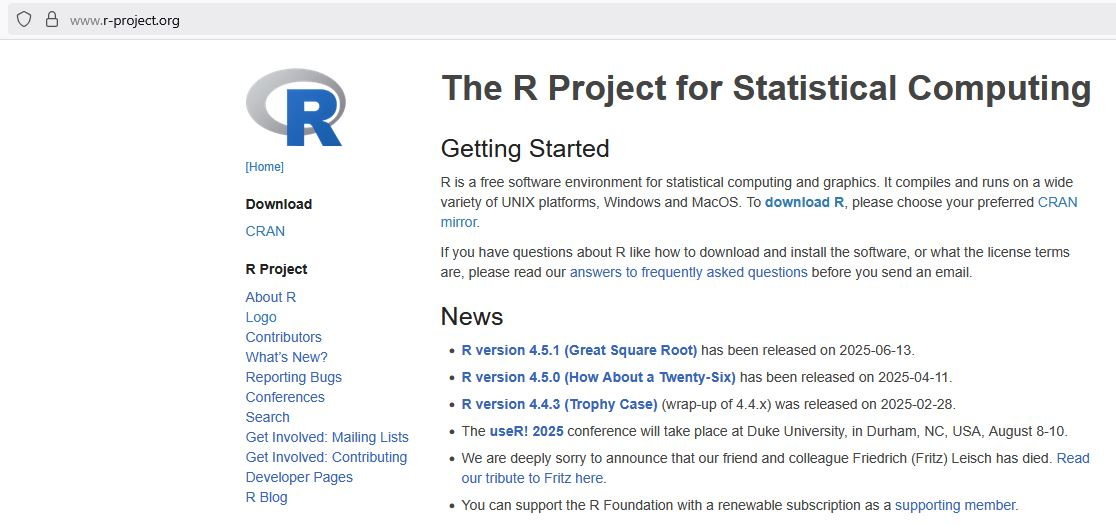
\includegraphics[width=1\linewidth]{./images/telecharger_R_1} 

}

\caption{Site du R project, en juillet 2025}\label{fig:dlR1}
\end{figure}

Cliquez sur ``download R'', choisissez un site mirroir (par exemple un des sites en France).

Puis téléchargez la version de R en fonction de votre système d'exploitation (Windows, macOS ou Linux).

\begin{figure}

{\centering 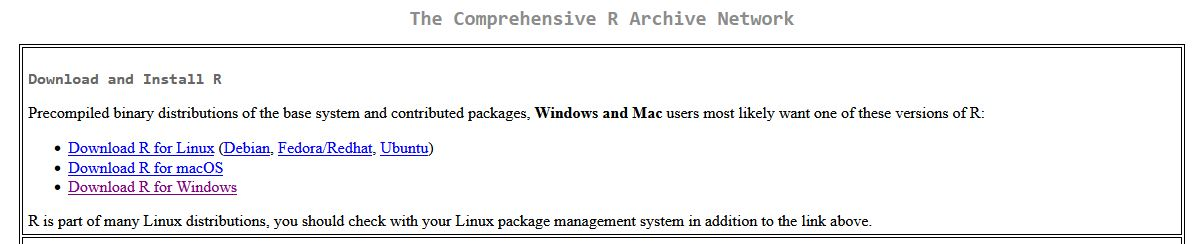
\includegraphics[width=1\linewidth]{./images/telecharger_R_2} 

}

\caption{Choisissez la version adaptée à votre système d'exploitation}\label{fig:dlR2}
\end{figure}

Enfin, installez R à partir du fichier d'installation que vous venez de télécharger.

\subsection{Ouvrez le logiciel R}\label{ouvrez-le-logiciel-r}

Si vous ouvrez le logiciel R, vous aller trouver l'interface graphique de R (\emph{RGui} pour \emph{R Graphical user interface}). Il est possible de faire vos analyses statistiques à partir de cette interface graphique, mais elle est très très austère.

\begin{figure}

{\centering 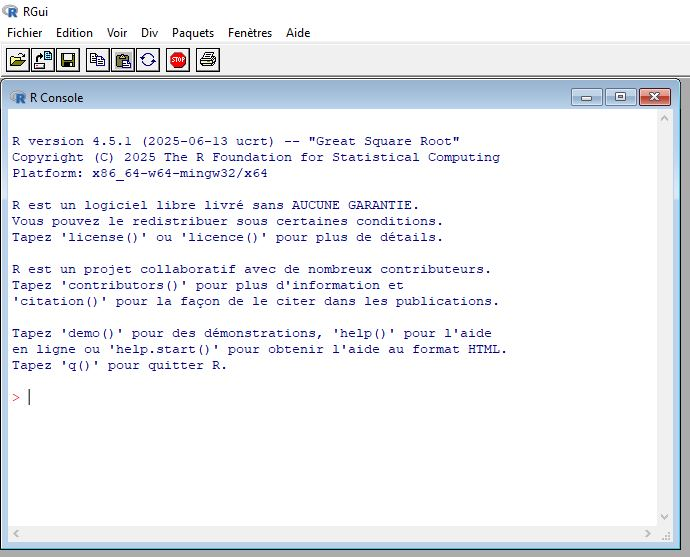
\includegraphics[width=0.5\linewidth]{./images/Rgui} 

}

\caption{L'interface graphique de R (RGui)}\label{fig:RGui}
\end{figure}

Plutôt que d'utiliser cette interface RGui, nous vous recommandons fortement d'utiliser un Environnement de Développement Intégré (IDE), comme RStudio, qui vous facilitera grandement la vie pour utiliser un logiciel statistique qui repose sur de la programmation.

\section{Téléchargez un IDE (RStudio recommandé)}\label{tuxe9luxe9chargez-un-ide-rstudio-recommanduxe9}

RStudio est un environnement qui permet d'utiliser R, mais également d'autres logiciels de programmation comme Python, SQL, Stan, C++, etc. Cet environnement vous facilitera le travail pour :

\begin{itemize}
\tightlist
\item
  éditer vos scripts de programmation,
\item
  accéder à la console,
\item
  visualiser vos environnements de travail avec les fichiers et les objets qu'il contient,
\item
  visualiser vos sorties graphiques et certaines tables d'analyses,
\item
  visualiser vos données,
\item
  visualiser les fichiers d'aide,
\item
  gérer les \emph{packages} permettant de faire des analyses spécifiques,
\item
  et bien d'autres choses encore.
\end{itemize}

Par exemple, le tutoriel que vous êtes en train de lire a été créé à partir du package \href{https://bookdown.org/}{\texttt{bookdown}} avec le logiciels R, au sein de l'IDE RStudio,

Vous pouvez télécharger la dernière version de \href{https://posit.co/download/rstudio-desktop/}{RStudio} sur le site de la compagnie \href{https://posit.co/products/open-source/rstudio/?sid=1}{Posit}. Choisissez la version qui est adaptée à votre système d'exploitation (Windows, macOS ou Linux).

\begin{figure}

{\centering 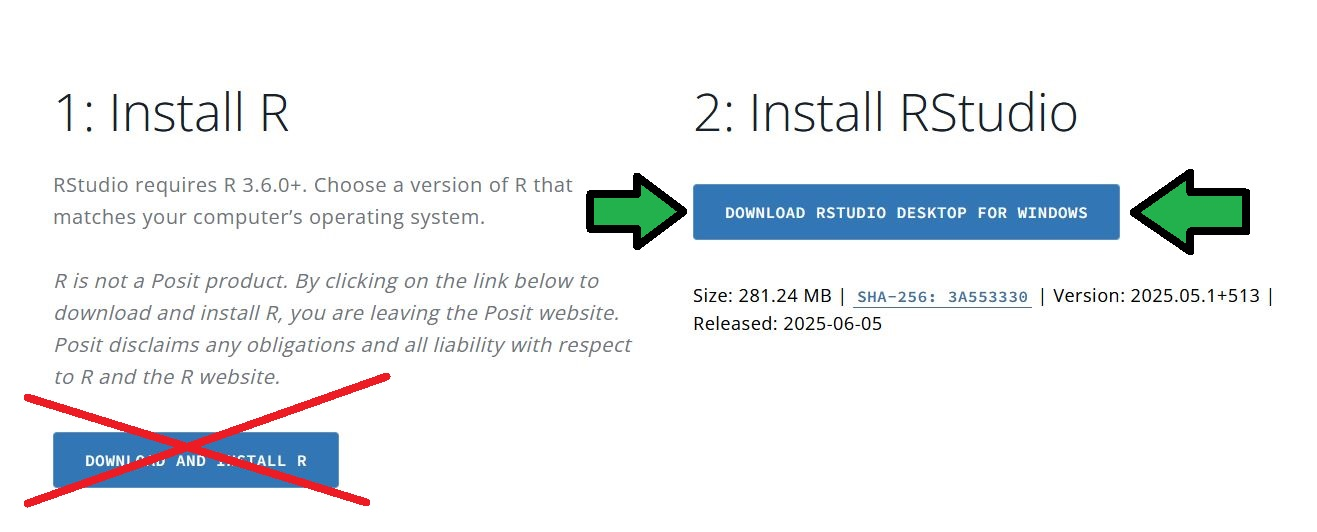
\includegraphics[width=1\linewidth]{./images/telecharger_RStudio_1} 

}

\caption{téléchargez RStudio}\label{fig:dlRStudio-1}
\end{figure}
\begin{figure}

{\centering 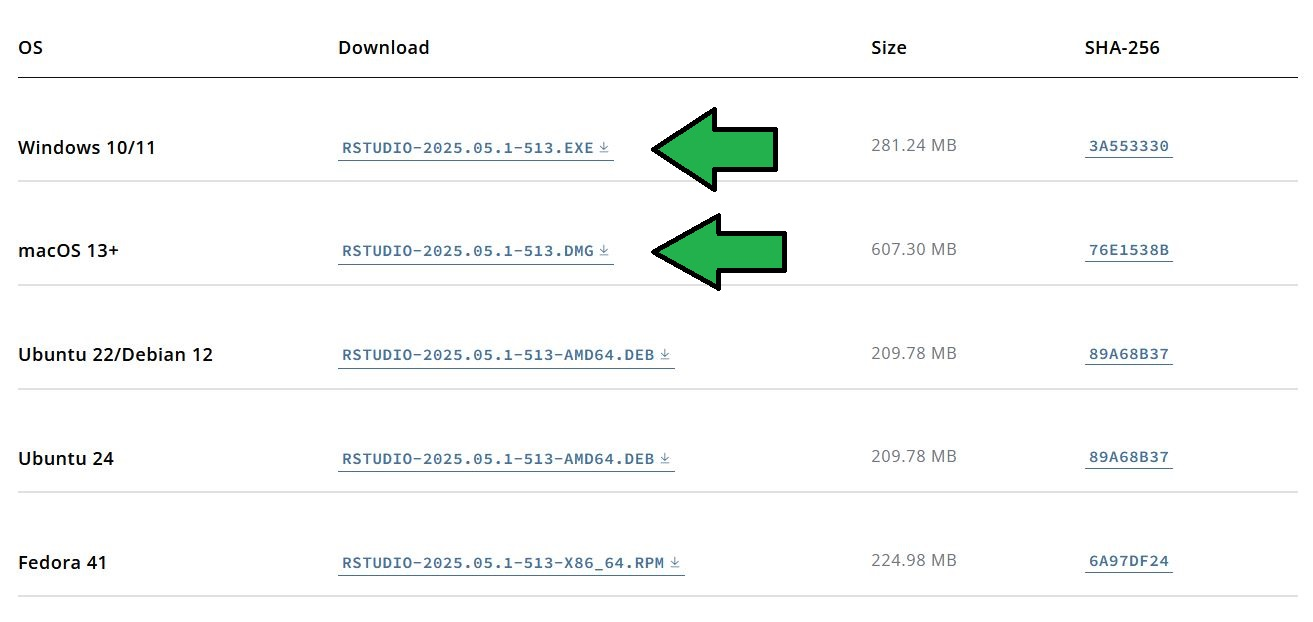
\includegraphics[width=1\linewidth]{./images/telecharger_RStudio_2} 

}

\caption{téléchargez RStudio}\label{fig:dlRStudio-2}
\end{figure}

Puis, installez RStudio à partir du fichier d'installation que vous venez de télécharger.

\subsection{Ouvrez l'IDE RStudio}\label{ouvrez-lide-rstudio}

Ouvrez RStudio, puis commencez par ouvrir un \textbf{script}

\begin{itemize}
\tightlist
\item
  à partir du menu File \textgreater{} New File \textgreater{} R script
\item
  ou bien en utilisant le raccourci Ctrl+Maj+N sur windows
\item
  ou bien en cliquant sur le petit fichier blanc avec un + vert en haut à gauche, puis choisir ``R script''
\end{itemize}

\begin{figure}

{\centering 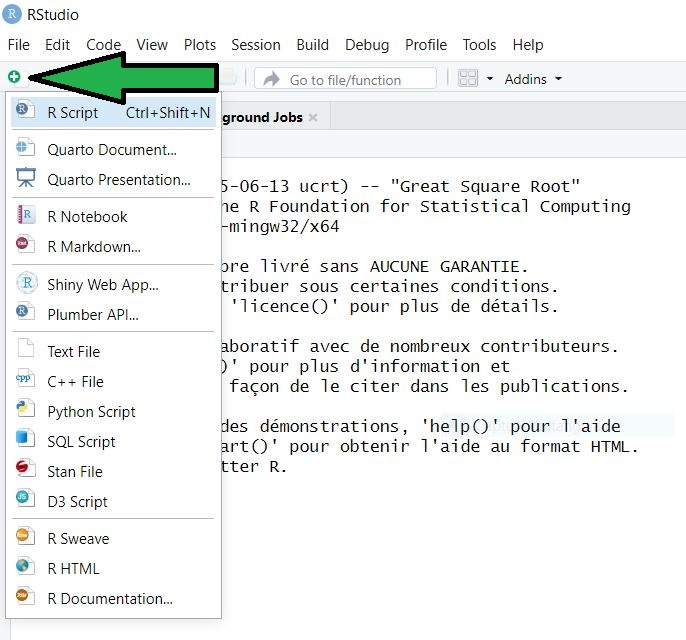
\includegraphics[width=0.5\linewidth]{./images/newscriptR} 

}

\caption{Ouvrir un nouveau script}\label{fig:newscript}
\end{figure}

L'interface de RStudio contient un menu, 4 quadrants et des sous-menus et boutons dans chaque cadrant.

\begin{figure}

{\centering 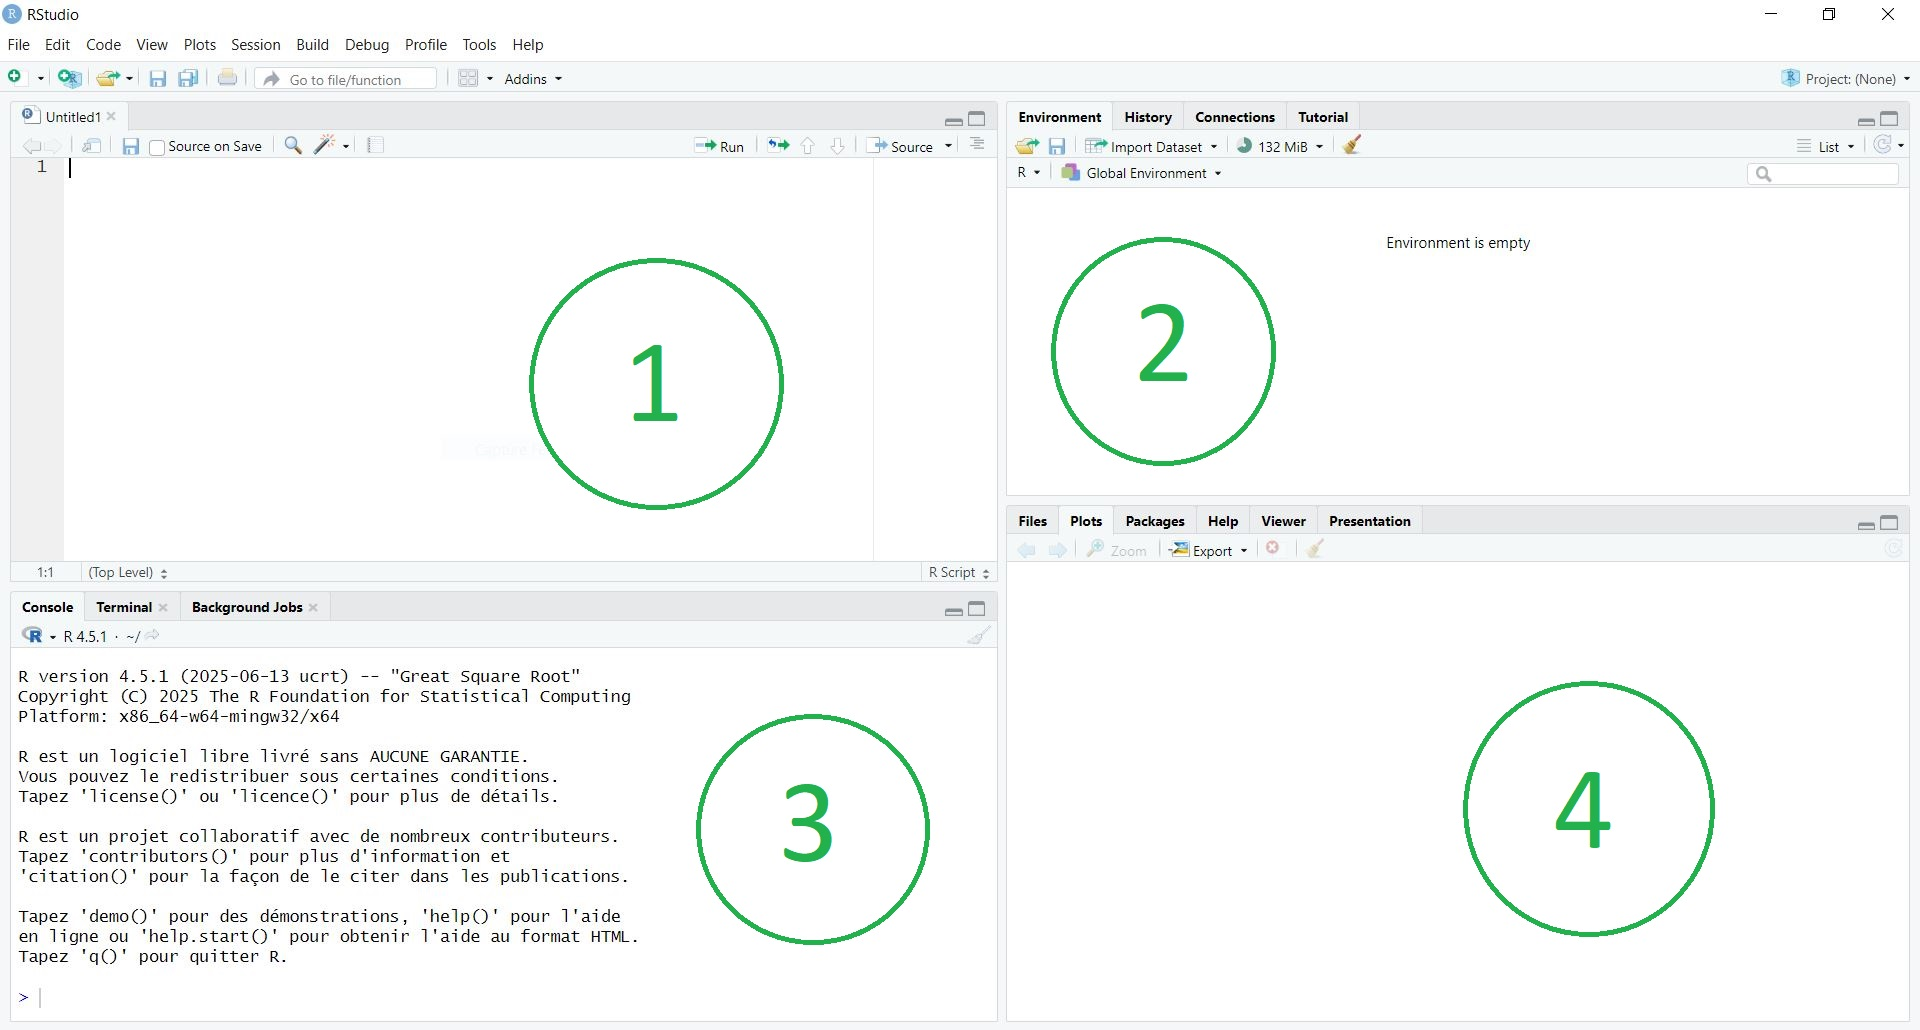
\includegraphics[width=1\linewidth]{./images/cadrants_RStudio} 

}

\caption{Les 4 cadrants de RStudio}\label{fig:RStudcadrants}
\end{figure}

Les menus qui vous seront le plus utiles sont :

\begin{itemize}
\tightlist
\item
  Dans le menu principal,

  \begin{itemize}
  \tightlist
  \item
    le menu \emph{File} vous permettra de créer de nouveaux fichiers, d'ouvrir des fichiers déjà existants, de sauver vos fichiers, d'importer des bases de données, etc.
  \item
    le menu \emph{Tools \textgreater{} Install packages\ldots{}} pour installer de nouveaux packages
  \item
    le menu \emph{Tools \textgreater{} Global Options\ldots{}} vous permet de choisir la version du logiciel R à utiliser (onglet ``R General'') ou bien de changer l'aspect graphique de l'environnement RStudio (onglet ``Appearance'', puis choisissez un ``Editor theme'', avec différentes interfaces claires ou sombres)
  \end{itemize}
\item
  Au sein du \textbf{script} (cadrant 1)

  \begin{itemize}
  \tightlist
  \item
    le bouton ``disquette'' permet de sauvegarder votre script
  \item
    le bouton ``run'' permet de faire tourner votre programme d'analyse (les lignes que vous avez sélectionnées). Par exemple, tapez la commande suivante dans le script, sélectionnez la ligne et cliquez sur le bouton ``run'' (ou avec un raccourci clavier \texttt{ctrl}+\texttt{entrée} sur windows, ou encore \texttt{command}+\texttt{entrée} sur macOS).
  \end{itemize}
\end{itemize}

\begin{Shaded}
\begin{Highlighting}[]
\FunctionTok{print}\NormalTok{(}\StringTok{"Hello Toulouse"}\NormalTok{)}
\end{Highlighting}
\end{Shaded}

et vous devriez voir la commande \texttt{\textgreater{}\ print("Hello\ Toulouse")} puis son résultat \texttt{"Hello\ Toulouse"} dans l'onglet \textbf{console} du cadrant 3.

\begin{itemize}
\tightlist
\item
  Au sein du cadrant 3, l'onglet le plus utile pour pour les débutants est l'onglet \textbf{console}

  \begin{itemize}
  \tightlist
  \item
    la console est la même que la console affichée dans l'interface RGui du logiciel R que l'on a vu au paragraphe 1.2.1.
  \item
    la console commence par afficher la version de R en cours d'utilisation
  \item
    vous pouvez y saisir des commandes et obtenir directement leurs résultats, par exemple si vous tapez dans la console \texttt{4+9}, vous obtiendrez directement le résultat \texttt{13}. \textbf{Attention, les commandes que vous saisissez directement dans la console ne seront pas sauvegardées. Si vous voulez sauvegarder des commandes, il faut utiliser le \emph{script} (cadrant 1)}
  \end{itemize}
\end{itemize}

\begin{Shaded}
\begin{Highlighting}[]
\DecValTok{4}\SpecialCharTok{+}\DecValTok{9}
\end{Highlighting}
\end{Shaded}

\begin{verbatim}
## [1] 13
\end{verbatim}

\begin{itemize}
\tightlist
\item
  Au sein du cadrant 2, l'onglet le plus utile pour les débutants est l'onglet \textbf{Environment}

  \begin{itemize}
  \tightlist
  \item
    cet onglet vous permettra de visualiser les ``objets R'' créés pendant vos analyses.
  \item
    Par exemple si vous saisissez \texttt{v\ \textless{}-\ 1:10} dans la console, vous allez voir apparaître l'objet \texttt{v} dans l'environnement de travail (il s'agit d'un vecteur de 1 à 10, nommé ``v'').
  \end{itemize}
\item
  Au sein du cadrant 4, les onglets les plus utiles pour les débutants sont :

  \begin{itemize}
  \tightlist
  \item
    l'onglet ``File'' qui contient les dossiers et fichiers au sein d'un dossier de travail (voir le chapitre 3 pour créer et organiser un dossier de travail associé à un ``projet R'')
  \item
    l'onglet ``Plots'' où vous retrouverez vos sorties graphiques. Au sein de cet onglet, vous trouverez un menu pour exporter vos graphiques selon différents formats. Des boutons permettent également de zoomer et d'effacer les graphiques. Par exemple, si vous saisissez \texttt{hist(rnorm(10000))} dans la console, un histogramme d'une distribution normale centrée réduite va apparaître. Vous pouvez effacer la figure en cliquant sur le bouton avec la croix rouge (efface la figure actuelle) ou le balet (efface l'ensemble des figures).
  \item
    l'onglet ``Packages'' où vous pourrez activer, désactiver ou mettre à jour les packages qui ont été téléchargés.
  \item
    l'onglet ``Help'' où vous trouverez de l'aide. Par exemple si vous saisissez \texttt{help(mean)} dans la console, l'aide de la commande \texttt{mean} va s'afficher. Vous pouvez également utiliser le champ de recherche de fonctions dans le menu ``Help''.
  \end{itemize}
\end{itemize}

\section{Trouver de l'aide sur R}\label{trouver-de-laide-sur-r}

De nombreuses ressources sont disponibles pour vous aider à utiliser R :

\begin{itemize}
\item
  Les pages d'aide en ligne de R, qui apparaîssent directement dans RStudio. Vous pouvez obtenir de l'aide sur des fonctions et des packages :

  \begin{itemize}
  \tightlist
  \item
    en appliquant une recherche par mot clé dans le champ de recherche de l'onglet ``help''
  \item
    en utilisant directement dans la console la fonction \texttt{help.search()} ou \texttt{??} associée à un mot clé (par exemple \texttt{help.search(student)} ou \texttt{??student}), ou la fonction \texttt{help()} associée à une fonction (par exemple \texttt{help(t.test)} ou \texttt{?t.test})
  \item
    Ces pages d'aide suivent la structure suivante :

    \begin{itemize}
    \tightlist
    \item
      une partie ``Description'' qui décrit en quelques phrases ce que fait la fonction
    \item
      une partie ``Usage'' qui décrit la syntaxe de la fonction avec ses arguments
    \item
      une partie ``Argument'' qui précise comment renseigner les arguments de la fonction
    \item
      une partie ``Detail'' qui décrit en détail comment utiliser la fonction et ses arguments
    \item
      une partie ``Value'' qui décrit les sorties (les résultats) de la fonction, avec les éventuels sous-objets de la sortie
    \item
      une partie ``Exemples'' qui indique quelques exemple que vous pouvez directement lancer en cliquant sur ``Run examples''
    \end{itemize}
  \end{itemize}
\item
  Des fiches ``mémoires'' \emph{cheat sheets} qui résument les principales fonctions :

  \begin{itemize}
  \tightlist
  \item
    pour les \href{https://rstudio.github.io/cheatsheets/base-r.pdf}{commandes R bases}
  \item
    des \href{https://rstudio.github.io/cheatsheets/R-best-practice.pdf}{bonnes pratiques sur R}
  \item
    méthodes de visualisation avec le package \href{https://posit.co/wp-content/uploads/2022/10/data-visualization-1.pdf}{ggplot2}
  \item
    l'utilisation du package \href{https://rstudio.github.io/cheatsheets/datatable.pdf}{data.table}
  \item
    l'utilisation du package \href{https://dplyr.tidyverse.org/}{dplyr} et sa \href{https://github.com/rstudio/cheatsheets/blob/main/data-transformation.pdf}{fiche dplyr}
  \item
    l'utilisation du package \href{https://rstudio.github.io/cheatsheets/html/strings.html}{stringr} pour manipuler les chaînes de caractères, avec la \href{https://rstudio.github.io/cheatsheets/strings.pdf}{fiche stringr}
  \item
    la manipulation de dates \href{https://rstudio.github.io/cheatsheets/html/lubridate.html}{Dates and times with lubridate} et la \href{https://rstudio.github.io/cheatsheets/lubridate.pdf}{fiche lubridate}
  \end{itemize}
\item
  De nombreux livres et tutoriels disponibles gratuitement en ligne :

  \begin{itemize}
  \tightlist
  \item
    Le \href{https://larmarange.github.io/guide-R/}{guide R} de Joseph Larmarange, est un guide très complet et didactique, en français
  \item
    L'\href{https://epirhandbook.com/en/index.html}{Epidemiologist R Handbook} est un tutoriel en anglais pour l'utilisation de R par des épidémiologistes
  \item
    Software carpentry met à disposition des guides introductifs bien réalisés en anglais, par exemple \href{https://swcarpentry.github.io/r-novice-gapminder/}{R for Reproducible Scientific Analysis} ou encore \href{https://swcarpentry.github.io/r-novice-inflammation/}{Programming with R}
  \item
    le livre \href{https://r4ds.hadley.nz/}{R for Data Science} propose une introduction très complète pour l'analyse de données descriptive principalement basée sur la suite de packages du \href{https://www.tidyverse.org/}{Tidyverse}
  \item
    le package R \href{https://swirlstats.com/}{swirl} propose une formation interactive directement dans la console de RStudio, téléchargez le package (\texttt{install.packages("swirl")}), chargez le package (\texttt{library("swirl")}) et laissez vous guider après avoir saisi \texttt{swirl()} dans la console.
  \item
    \href{https://education.rstudio.com/learn/beginner/}{RStudio Education} liste plusieurs ressources intéressantes pour les débutants
  \item
    Le site CRAN a des manuels assez complets, par exemple la page \href{https://cran.r-project.org/doc/manuals/R-lang.html}{R Language Definition} est une introduction assez complète au langage de programmation R. La page \href{https://cran.r-project.org/web/views/}{CRAN Task Views} liste les packages qui sont disponibles par thématique ou type d'anlayse.
  \end{itemize}
\item
  Rechercher à l'aide d'un moteur de recherche (google, DuckDuckGo, Bing, etc). Ces recherches vous amèneront régulièrement vers des forums de discussion comme \href{https://stackoverflow.com/questions/tagged/R}{stackoverflow} ou \href{https://stats.stackexchange.com/questions/tagged/r}{stackExchange}. Si vous rencontrez une erreur ou une difficulté, il y a toutes les chances que d'autres personnes aient déjà rencontré ces erreurs et difficultés avant vous, et que des solutions détaillées soient proposées dans ces forums.
\item
  Les chatbots de type GPT, Copilot ou Gemini : dans le cadre de votre formation au logiciel R, nous vous déconseillons l'utilisation de ces outils basés sur des LLM. Ces outils posent de nombreux problèmes en termes de transparence, de respect de droit d'auteur, d'impact environnemental, de déqualification (délegation de compétences pour rechercher de l'information, perte d'esprit critique), de dépendance aux Gafams, de dégradation des systèmes d'information, etc. Par ailleurs, bien qu'ils peuvent apporter des solutions fonctionnelles, il est bien plus utile d'avoir une bonne compréhension des bases de programmations sur R avant d'utiliser de tels outils : sans une bonne compréhension de la logique de programmation et des principales fonctions de R, vous aurez des difficultés à évaluer la fiabilité des solutions proposées, à vous débloquez en cas de problèmes, ou encore à adapter vos prompts pour obtenir de meilleures réponses. Les ressources décrites précédemment devraient vous permettre d'apporter efficacement des réponses à vos questions.
\end{itemize}

\section{Conventions d'écriture}\label{conventions-duxe9criture}

Certaines conventions ont été proposées pour faciliter l'écriture et la lecture du code de programmation dans R. Elles ne sont pas obligatoires, mais nous vous encourrageons à les suivre.

Par exemple, le \href{https://style.tidyverse.org/}{\emph{Tidyverse style guide}} :

\begin{itemize}
\tightlist
\item
  nommer les variables et les fonctions en lettres minuscules, à l'aide de mots et de chiffres séparés par \texttt{\_} (\emph{underscore}). Par exemple \texttt{csp\_1}. Cette convention fait référence au style \href{https://en.wikipedia.org/wiki/Snake_case}{``snake case''}
\item
  ajouter un espace après une virgule, par exemple \texttt{x{[}2,\ 5{]}}
\item
  ajouter des espaces avant et après les opérateurs arithmétiques, par exemple \texttt{x\ \textless{}-\ (1\ +\ 2)\ /\ 5}, à quelques exceptions près (pas d'espace avant ou après le signe ``puissance'' \texttt{\^{}}) \texttt{y\ \textless{}-\ x\^{}2\ +\ 3}
\end{itemize}

\chapter{Les objets dans R}\label{les-objets-dans-r}

\section{Manipuler les objets dans l'environnement}\label{manipuler-les-objets-dans-lenvironnement}

La programmation R repose sur des \emph{objets}, qui apparaîtront dans la fenêtre \emph{Environment} de RStudio.

Voici quelques commandes de gestion des objets dans votre environnement :

\begin{itemize}
\tightlist
\item
  dans la console, commencez par créer les objets suivants. Pour \textbf{assigner une ou plusieurs valeurs à un objet}, on utilise une flèche dirigée vers la gauche \texttt{\textless{}-}. Vous verrez apparaître ces objets dans la fenêtre \emph{Environment}.
\end{itemize}

\begin{Shaded}
\begin{Highlighting}[]
\CommentTok{\# note : le signe dièze (\#) permet d\textquotesingle{}ajouter des commentaires dans le code  }
\CommentTok{\# {-} le 1er objet est un vecteur de 10 entiers de 1 à 10}
\CommentTok{\# {-} le 2ème objet est un vecteur de 3 lettres A, B et C}
\CommentTok{\# {-} le 3ème objet est un vecteur de 2 réels, calculés par 2 opérations}
\CommentTok{\# {-} le 4ème objet est une fonction qui ajoute 2 au vecteur x}
\CommentTok{\# {-} le 5ème objet est un scalaire égal à 42}
\NormalTok{objet\_1 }\OtherTok{\textless{}{-}} \FunctionTok{c}\NormalTok{(}\DecValTok{1}\SpecialCharTok{:}\DecValTok{10}\NormalTok{) }
\NormalTok{objet\_2 }\OtherTok{\textless{}{-}} \FunctionTok{c}\NormalTok{(}\StringTok{"A"}\NormalTok{,}\StringTok{"B"}\NormalTok{,}\StringTok{"C"}\NormalTok{) }
\NormalTok{objet\_3 }\OtherTok{\textless{}{-}} \FunctionTok{c}\NormalTok{(}\DecValTok{10} \SpecialCharTok{/} \DecValTok{3}\NormalTok{, }\DecValTok{4} \SpecialCharTok{*} \DecValTok{5}\NormalTok{) }
\NormalTok{objet\_4 }\OtherTok{\textless{}{-}} \ControlFlowTok{function}\NormalTok{(x) \{x }\SpecialCharTok{+} \DecValTok{2}\NormalTok{\} }
\NormalTok{objet\_5 }\OtherTok{\textless{}{-}} \DecValTok{42} 
\end{Highlighting}
\end{Shaded}

\begin{itemize}
\tightlist
\item
  la commande \texttt{ls()} permet de \textbf{lister} les objets dans l'environnement.
\item
  la commande \texttt{rm()} permet de \textbf{supprimer} (\emph{remove}) un ou plusieurs objets de l'environnement.
\end{itemize}

\begin{Shaded}
\begin{Highlighting}[]
\FunctionTok{ls}\NormalTok{()}
\end{Highlighting}
\end{Shaded}

\begin{verbatim}
## [1] "objet_1" "objet_2" "objet_3" "objet_4" "objet_5"
\end{verbatim}

\begin{Shaded}
\begin{Highlighting}[]
\FunctionTok{rm}\NormalTok{(objet\_2,objet\_5)}
\FunctionTok{rm}\NormalTok{(}\AttributeTok{list =} \FunctionTok{ls}\NormalTok{()) }\CommentTok{\# pour supprimer tous les objets présents dans l\textquotesingle{}environnement}
\end{Highlighting}
\end{Shaded}

\section{Principaux types de données}\label{principaux-types-de-donnuxe9es}

Les données peuvent être de différents types :

\begin{itemize}
\tightlist
\item
  des \textbf{nombres} (\texttt{?numeric}). Ces nombres peuvent être des \textbf{nombres réels} (\texttt{?double}), par exemple \texttt{12.43}. Il peut également s'agir de \textbf{nombres entiers} (\texttt{?integer}). Les nombres entiers sont saisis en ajoutant \texttt{L} à droite du nombre, par exemple \texttt{5L}.
\item
  des \textbf{chaînes de caractères textuels} (\texttt{?character}), définis avec des guillemets simples ou doubles , par exemple \texttt{\textquotesingle{}bonjour\textquotesingle{}} ou \texttt{"au\ revoir"}
\item
  des \textbf{valeurs logiques} (\texttt{?logical}), avec deux valeurs possibles :

  \begin{itemize}
  \tightlist
  \item
    valeur booléenne \emph{vraie}, notée \texttt{TRUE} ou bien \texttt{T}
  \item
    valeur booléenne \emph{fausse}, notée \texttt{FALSE} ou bien \texttt{F}
  \end{itemize}
\item
  des \textbf{variables qualitatives nominales} (\texttt{?factor}) ou \textbf{ordinales} (\texttt{?ordered})
\item
  des \textbf{dates} (\texttt{?Date})
\item
  etc.
\item
  une \textbf{valeur manquante} se note \texttt{NA}. L'\textbf{ensemble vide} se note \texttt{NULL}
\end{itemize}

\subsection{\texorpdfstring{Décrire le type de l'objet \(\spadesuit\)}{Décrire le type de l'objet \textbackslash spadesuit}}\label{duxe9crire-le-type-de-lobjet-spadesuit}

On peut décrire quel est le type de l'objet avec les fonctions \texttt{typeof} (le type le plus élémentaire), \texttt{mode} et \texttt{storage.mode} (type de l'objet et mode de stockage de l'objet selon un regroupement un peu plus large)

\begin{Shaded}
\begin{Highlighting}[]
\CommentTok{\# les valeurs réelles (\textquotesingle{}double\textquotesingle{}) et les entiers (\textquotesingle{}integer\textquotesingle{}) sont de mode \textquotesingle{}numeric\textquotesingle{}}
\FunctionTok{typeof}\NormalTok{(}\FloatTok{2.53}\NormalTok{) }\CommentTok{\# un réel}
\FunctionTok{typeof}\NormalTok{(}\DecValTok{5}\DataTypeTok{L}\NormalTok{) }\CommentTok{\# et un entier}
\FunctionTok{mode}\NormalTok{(}\FloatTok{2.53}\NormalTok{) }\CommentTok{\# sont de type \textquotesingle{}numeric\textquotesingle{}}
\FunctionTok{mode}\NormalTok{(}\DecValTok{5}\DataTypeTok{L}\NormalTok{)}
\FunctionTok{storage.mode}\NormalTok{(}\FloatTok{2.53}\NormalTok{)}
\FunctionTok{storage.mode}\NormalTok{(}\DecValTok{5}\DataTypeTok{L}\NormalTok{)}

\CommentTok{\# les chaînes de caractères sont de type et de mode \textquotesingle{}character\textquotesingle{}}
\FunctionTok{typeof}\NormalTok{(}\FunctionTok{c}\NormalTok{(}\StringTok{"hello"}\NormalTok{,}\StringTok{"Toulouse"}\NormalTok{))}
\FunctionTok{mode}\NormalTok{(}\FunctionTok{c}\NormalTok{(}\StringTok{"hello"}\NormalTok{,}\StringTok{"Toulouse"}\NormalTok{))}

\CommentTok{\# les valeurs logiques sont de type \textquotesingle{}logical\textquotesingle{}}
\FunctionTok{typeof}\NormalTok{(}\FunctionTok{c}\NormalTok{(}\ConstantTok{TRUE}\NormalTok{,}\ConstantTok{FALSE}\NormalTok{,}\ConstantTok{FALSE}\NormalTok{))}
\FunctionTok{mode}\NormalTok{(}\FunctionTok{c}\NormalTok{(}\ConstantTok{TRUE}\NormalTok{,}\ConstantTok{FALSE}\NormalTok{,}\ConstantTok{FALSE}\NormalTok{))}
\end{Highlighting}
\end{Shaded}

\begin{longtable}[]{@{}
  >{\centering\arraybackslash}p{(\linewidth - 6\tabcolsep) * \real{0.3205}}
  >{\centering\arraybackslash}p{(\linewidth - 6\tabcolsep) * \real{0.2308}}
  >{\centering\arraybackslash}p{(\linewidth - 6\tabcolsep) * \real{0.2051}}
  >{\centering\arraybackslash}p{(\linewidth - 6\tabcolsep) * \real{0.2436}}@{}}
\toprule\noalign{}
\begin{minipage}[b]{\linewidth}\centering
\texttt{x}
\end{minipage} & \begin{minipage}[b]{\linewidth}\centering
\texttt{typeof(x)}
\end{minipage} & \begin{minipage}[b]{\linewidth}\centering
\texttt{mode(x)}
\end{minipage} & \begin{minipage}[b]{\linewidth}\centering
\texttt{storage.mode(x)}
\end{minipage} \\
\midrule\noalign{}
\endhead
\bottomrule\noalign{}
\endlastfoot
\texttt{2.53} & \texttt{"double"} & \texttt{"numeric"} & \texttt{"double"} \\
\texttt{5L} & \texttt{"integer"} & \texttt{"numeric"} & \texttt{"integer"} \\
\texttt{"bonjour"} & \texttt{"character"} & \texttt{"character"} & \texttt{"character"} \\
\texttt{TRUE} & \texttt{"logical"} & \texttt{"logical"} & \texttt{"logical"} \\
\texttt{as.Date("2025-07-01")} & \texttt{"double"} & \texttt{"numeric"} & \texttt{"double"} \\
\end{longtable}

Les fonctions \texttt{as.numeric}, \texttt{as.integer}, \texttt{as.character}, \texttt{as.logical} permettent de définir un objet \emph{en tant que} numérique, entier, chaîne de caractères, logique.

\begin{Shaded}
\begin{Highlighting}[]
\FunctionTok{as.numeric}\NormalTok{(}\DecValTok{5}\DataTypeTok{L}\NormalTok{) }\CommentTok{\# définit un nombre entier en tant que nombre réel}
\FunctionTok{as.integer}\NormalTok{(}\FloatTok{4.95}\NormalTok{) }\CommentTok{\# définit un réel en tant qu\textquotesingle{}entier, seul l\textquotesingle{}entier est conservé}
\FunctionTok{as.character}\NormalTok{(}\FloatTok{4.95}\NormalTok{) }\CommentTok{\# définit un nombre en tant que chaîne de caractères}

\CommentTok{\# définir une valeur logique TRUE et FALSE en tant que valeur numérique }
\CommentTok{\# ou en tant qu\textquotesingle{}entier donne les valeurs 1 et 0, respectivement}
\FunctionTok{as.numeric}\NormalTok{(}\ConstantTok{TRUE}\NormalTok{) }
\FunctionTok{as.numeric}\NormalTok{(}\ConstantTok{FALSE}\NormalTok{) }

\CommentTok{\# définir le nombre 0 en tant que valeur logique donne la valeur FALSE}
\FunctionTok{as.logical}\NormalTok{(}\DecValTok{0}\NormalTok{)}

\CommentTok{\# définir tout nombre différent de 0 en tant que valeur logique }
\CommentTok{\# donne la valeur TRUE}
\FunctionTok{as.logical}\NormalTok{(}\SpecialCharTok{{-}}\DecValTok{14}\NormalTok{)}
\FunctionTok{as.logical}\NormalTok{(}\DecValTok{1}\NormalTok{)}
\FunctionTok{as.logical}\NormalTok{(}\FloatTok{4.95}\NormalTok{)}
\end{Highlighting}
\end{Shaded}

Les fonctions \texttt{is.numeric}, \texttt{is.integer}, \texttt{is.character}, \texttt{is.logical} permettent d'évaluer si un objet est de type numérique, entier, textuel, logique.

\begin{Shaded}
\begin{Highlighting}[]
\FunctionTok{is.numeric}\NormalTok{(}\DecValTok{5}\DataTypeTok{L}\NormalTok{) }\CommentTok{\# TRUE, un entier est bien un objet numérique}
\FunctionTok{is.integer}\NormalTok{(}\FloatTok{4.95}\NormalTok{) }\CommentTok{\# FALSE, 4.95 n\textquotesingle{}est pas un entier}
\FunctionTok{is.numeric}\NormalTok{(}\StringTok{"bonjour"}\NormalTok{) }\CommentTok{\# FALSE "bonjour" est une chaîne de caractères}
\FunctionTok{is.character}\NormalTok{(}\StringTok{"bonjour"}\NormalTok{) }\CommentTok{\# TRUE, "bonjour" est bien une chaîne de caractères}
\FunctionTok{is.character}\NormalTok{(}\FloatTok{4.95}\NormalTok{) }\CommentTok{\# FALSE, 4.95 est un objet numérique}
\FunctionTok{is.logical}\NormalTok{(}\DecValTok{1}\NormalTok{) }\CommentTok{\# FALSE, 1 est un objet numérique}
\FunctionTok{is.logical}\NormalTok{(}\FunctionTok{as.logical}\NormalTok{(}\DecValTok{1}\NormalTok{)) }\CommentTok{\# TRUE, as.logical(1) = TRUE, qui est un objet logique}
\FunctionTok{is.logical}\NormalTok{(}\ConstantTok{TRUE}\NormalTok{) }\CommentTok{\# TRUE est bien un objet logique}
\end{Highlighting}
\end{Shaded}

\section{Principales structures de données}\label{principales-structures-de-donnuxe9es}

Les principales structures de données que nous allons détailler dans la suite de ce chapitre sont :

\begin{itemize}
\tightlist
\item
  les vecteurs (\texttt{?vector}), dont font partie les scalaires (vecteurs à une seule valeur).
\item
  les matrices (\texttt{?matrix}, \texttt{?array})
\item
  les listes (\texttt{?list})
\item
  les bases de données (\texttt{?data.frames}). Il existe d'autres formats de base de données qui seront présentés plus tard (avec les packages \texttt{tidyverse} et \texttt{data.table} par exemple)
\end{itemize}

\section{Objet à une seule valeur (scalaire ou texte)}\label{objet-uxe0-une-seule-valeur-scalaire-ou-texte}

\subsection{Scalaires}\label{scalaires}

Assignez les valeurs 4 et 5 à deux objets

\begin{Shaded}
\begin{Highlighting}[]
\NormalTok{x\_1 }\OtherTok{\textless{}{-}} \DecValTok{4}
\NormalTok{x\_2 }\OtherTok{\textless{}{-}} \DecValTok{5}
\end{Highlighting}
\end{Shaded}

\subsection{Opérations mathématiques sur les scalaires}\label{opuxe9rations-mathuxe9matiques-sur-les-scalaires}

\subsubsection{Calculatrice}\label{calculatrice}

On peut utiliser les opérations classiques, comme sur une calculatrice :

\begin{itemize}
\tightlist
\item
  \texttt{+} pour \textbf{additionner}
\item
  \texttt{-} pour \textbf{soustraire}
\item
  \texttt{*} pour \textbf{multiplier}
\item
  \texttt{/} pour \textbf{diviser}
\item
  \texttt{\^{}} pour mettre à la \textbf{puissance}
\item
  \texttt{e} pour la \textbf{notation scientifique}
\end{itemize}

\begin{Shaded}
\begin{Highlighting}[]
\NormalTok{x\_1 }\SpecialCharTok{+}\NormalTok{ x\_2 }\CommentTok{\# 4 + 5 = 9}
\DecValTok{10} \SpecialCharTok{{-}}\NormalTok{ x\_1 }\CommentTok{\# 10 {-} 4 = 6}
\NormalTok{x\_1 }\SpecialCharTok{*}\NormalTok{ x\_2 }\CommentTok{\#  4 * 5 = 20}
\DecValTok{20} \SpecialCharTok{/}\NormalTok{ x\_2 }\CommentTok{\# 20 / 5 = 4}
\NormalTok{x\_1}\SpecialCharTok{\^{}}\DecValTok{2} \CommentTok{\#  4\^{}2 = 16}
\DecValTok{10}\SpecialCharTok{\^{}{-}}\DecValTok{1} \CommentTok{\# 1/10 = 0.1}
\DecValTok{25}\SpecialCharTok{\^{}}\NormalTok{(}\FloatTok{0.5}\NormalTok{) }\CommentTok{\# racine carrée de 25 (puissance 1/2)}

\CommentTok{\# notation scientifique pour les grands et petits nombres}
\DecValTok{1}\SpecialCharTok{/}\DecValTok{1000000} \CommentTok{\# 1 pour 1 million = 1e{-}6}
\DecValTok{1}\SpecialCharTok{/}\FloatTok{1e6}
\FloatTok{1e6} \SpecialCharTok{*} \DecValTok{1000} \CommentTok{\# 1 million * 1000 = 1 milliard}
\end{Highlighting}
\end{Shaded}

\subsubsection{Fonctions mathématiques}\label{fonctions-mathuxe9matiques}

Plusieurs fonctions mathématiques de bases sont implémentées nativement dans R :

\begin{itemize}
\tightlist
\item
  \texttt{log(x)} ou \texttt{log(x,\ base\ =\ exp(1)} pour le \textbf{logarithme} népérien,
\item
  \texttt{log10(x)} pour le logarithme base 10, \texttt{log2(x)} pour le logarithme base 2,
\item
  \texttt{log(x,\ base\ =\ b)} pour le logarithme base \texttt{b},
\item
  \texttt{exp(x)} pour l'\textbf{exponentielle} de \texttt{x}
\item
  \texttt{sqrt(x)} pour la \textbf{racine carrée} de \texttt{x}
\item
  \texttt{abs(x)} pour la \textbf{valeur absolue} de \texttt{x}
\item
  les \textbf{fonctions trigonométriques} sont implémentées, avec \texttt{cos(x)}, \texttt{sin(x)}, \texttt{tan(x)} (cf.~\texttt{?Trig})
\item
  la \textbf{constante \(\pi\)} est implémentée avec \texttt{pi} (cf.~\texttt{?Constants})
\end{itemize}

Si vous appliquer une fonction à une valeur qui ne fait pas partie du domaine de définition de la fonction, le résultat sera une valeur manquante notée \texttt{NaN} (\emph{not a number}). Un message d'avertissement va apparaître si vous appliquez une fonction en dehors de son domaine de définition.

\begin{Shaded}
\begin{Highlighting}[]
\CommentTok{\# logarithmes et exponentielles}
\FunctionTok{log}\NormalTok{(}\DecValTok{1}\NormalTok{)}
\FunctionTok{log10}\NormalTok{(}\DecValTok{100}\NormalTok{)}
\FunctionTok{log}\NormalTok{(}\DecValTok{100}\NormalTok{, }\AttributeTok{base =} \DecValTok{10}\NormalTok{)}
\FunctionTok{exp}\NormalTok{(}\DecValTok{1}\NormalTok{)}

\CommentTok{\# racine carrée}
\FunctionTok{sqrt}\NormalTok{(x\_2}\SpecialCharTok{\^{}}\DecValTok{2}\NormalTok{)}

\CommentTok{\# valeur absolue}
\FunctionTok{abs}\NormalTok{(}\DecValTok{10}\NormalTok{)}
\FunctionTok{abs}\NormalTok{(}\SpecialCharTok{{-}}\DecValTok{10}\NormalTok{)}

\CommentTok{\# fonctions trigonométriques}
\FunctionTok{cos}\NormalTok{(}\DecValTok{1}\NormalTok{)}
\FunctionTok{sin}\NormalTok{(}\DecValTok{1}\NormalTok{)}
\FunctionTok{tan}\NormalTok{(}\DecValTok{1}\NormalTok{)}
\NormalTok{pi}
\DecValTok{2} \SpecialCharTok{*}\NormalTok{ pi }\SpecialCharTok{*} \DecValTok{10} \CommentTok{\# circonférence d\textquotesingle{}un cercle de rayon 10}

\CommentTok{\# si on utilise une valeur en dehors du domaine d\textquotesingle{}application de la fonction}
\FunctionTok{log}\NormalTok{(}\SpecialCharTok{{-}}\DecValTok{1}\NormalTok{) }\CommentTok{\# {-}1 est en dehors du domaine de définition de la fonction log}
\FunctionTok{sqrt}\NormalTok{(}\SpecialCharTok{{-}}\DecValTok{2}\NormalTok{) }\CommentTok{\# {-}2 est en dehors du domaine de définition de la fonction racine carrée}
\end{Highlighting}
\end{Shaded}

\subsubsection{\texorpdfstring{Fonctions d'arrondi \(\spadesuit\)}{Fonctions d'arrondi \textbackslash spadesuit}}\label{fonctions-darrondi-spadesuit}

Plusieurs fonctions sont disponibles dans R pour arrondir une valeur (cf.~\texttt{?Round}) :

\begin{itemize}
\tightlist
\item
  la fonction \texttt{round()} est utile pour arrondir les décimales. Il faut préciser en argument, le nombre de chiffres après la virgule. \textbf{Attention} : si le nombre se termine par un 5, l'arrondi se fait vers le chiffre pair le plus proche : 4.45 s'arrondit à 4.4 et 4.75 s'arrondit à 4.8
\item
  la fonction \texttt{signif()} arrondit aux chiffres les plus significatifs (les plus grands)
\item
  la fonction \texttt{floor()} arrondit la valeur à l'entier inférieur
\item
  la fonction \texttt{ceiling()} arrondit la valeur à l'entier supérieur
\item
  la fonction \texttt{trunc()}
\end{itemize}

\begin{Shaded}
\begin{Highlighting}[]
\DocumentationTok{\#\# fonction round()}
\CommentTok{\# l\textquotesingle{}argument digits permet de définir le nombre de chiffres après la virgule}
\CommentTok{\# exemple si vous voulez arrondir à 2 chiffres après la virgule}
\FunctionTok{round}\NormalTok{(}\FloatTok{0.09400}\NormalTok{, }\AttributeTok{digits =} \DecValTok{2}\NormalTok{)}
\FunctionTok{round}\NormalTok{(}\FloatTok{0.08600}\NormalTok{, }\AttributeTok{digits =} \DecValTok{2}\NormalTok{)}
\CommentTok{\# arroudir à 1 chiffre après la virgule}
\FunctionTok{round}\NormalTok{(}\FloatTok{4.450}\NormalTok{, }\AttributeTok{digits =} \DecValTok{1}\NormalTok{)}
\FunctionTok{round}\NormalTok{(}\FloatTok{4.750}\NormalTok{, }\AttributeTok{digits =} \DecValTok{1}\NormalTok{)}
\CommentTok{\# pour arrondir une valeur 5, le résultat va vers le chiffre pair le plus proche}
\FunctionTok{round}\NormalTok{(}\FloatTok{4.5}\NormalTok{, }\AttributeTok{digits =} \DecValTok{0}\NormalTok{) }\CommentTok{\# arrondit à l\textquotesingle{}entier pair le plus proche}
\FunctionTok{round}\NormalTok{(}\FloatTok{1.5}\NormalTok{, }\AttributeTok{digits =} \DecValTok{0}\NormalTok{) }\CommentTok{\# arrondit à l\textquotesingle{}entier pair le plus proche}

\DocumentationTok{\#\# fonction signif()}
\CommentTok{\# on garde les valeurs les plus significative, définie par l\textquotesingle{}argument digits}
\FunctionTok{signif}\NormalTok{(}\FloatTok{123.456789}\NormalTok{, }\AttributeTok{digits =} \DecValTok{1}\NormalTok{)}
\FunctionTok{signif}\NormalTok{(}\FloatTok{123.456789}\NormalTok{, }\AttributeTok{digits =} \DecValTok{2}\NormalTok{)}
\FunctionTok{signif}\NormalTok{(}\FloatTok{123.456789}\NormalTok{, }\AttributeTok{digits =} \DecValTok{3}\NormalTok{)}
\FunctionTok{signif}\NormalTok{(}\FloatTok{123.456789}\NormalTok{, }\AttributeTok{digits =} \DecValTok{4}\NormalTok{)}
\FunctionTok{signif}\NormalTok{(}\FloatTok{123.456789}\NormalTok{, }\AttributeTok{digits =} \DecValTok{5}\NormalTok{)}
\CommentTok{\# la règle d\textquotesingle{}arrondi vers le chiffre pair le plus proche est également appliquée}
\FunctionTok{signif}\NormalTok{(}\FloatTok{4.45}\NormalTok{, }\AttributeTok{digits =} \DecValTok{3}\NormalTok{)}
\FunctionTok{signif}\NormalTok{(}\FloatTok{4.45}\NormalTok{, }\AttributeTok{digits =} \DecValTok{2}\NormalTok{)}
\FunctionTok{signif}\NormalTok{(}\FloatTok{4.75}\NormalTok{, }\AttributeTok{digits =} \DecValTok{3}\NormalTok{)}
\FunctionTok{signif}\NormalTok{(}\FloatTok{4.75}\NormalTok{, }\AttributeTok{digits =} \DecValTok{2}\NormalTok{)}

\DocumentationTok{\#\# fonction trunc() supprime simplementles décimales}
\CommentTok{\# note : ici, il n\textquotesingle{}y a pas d\textquotesingle{}arrondi vers la chiffre pair la plus proche)}
\FunctionTok{trunc}\NormalTok{(}\FloatTok{123.456}\NormalTok{)}
\FunctionTok{trunc}\NormalTok{(}\FloatTok{4.5}\NormalTok{)}
\FunctionTok{trunc}\NormalTok{(}\FloatTok{1.5}\NormalTok{)}

\DocumentationTok{\#\# la fonction floor() arrondit à l\textquotesingle{}entier inférieur}
\FunctionTok{floor}\NormalTok{(}\FloatTok{4.1}\NormalTok{)}
\FunctionTok{floor}\NormalTok{(}\FloatTok{4.9}\NormalTok{)}

\DocumentationTok{\#\# la fonction ceiling() arrondit à l\textquotesingle{}entier supérieur}
\FunctionTok{ceiling}\NormalTok{(}\FloatTok{4.1}\NormalTok{)}
\FunctionTok{ceiling}\NormalTok{(}\FloatTok{4.9}\NormalTok{)}
\end{Highlighting}
\end{Shaded}

\subsection{Concaténation de chaînes de caractères}\label{concatuxe9nation-de-chauxeenes-de-caractuxe8res}

On peut concatener deux objets en chaînes de caractères :

\begin{itemize}
\tightlist
\item
  la fonction \texttt{paste()} concatène les chaînes de caractères en séparant les vecteurs par un espace (argument par défaut, cf \texttt{?paste}). Cet argument peut être modifié.
\item
  la fonction \texttt{paste0()} concatène les chaînes de caractères sans espace.
\end{itemize}

\begin{Shaded}
\begin{Highlighting}[]
\NormalTok{x1 }\OtherTok{\textless{}{-}} \StringTok{"Bonjour"}
\NormalTok{x2 }\OtherTok{\textless{}{-}} \StringTok{"Toulouse"}
\FunctionTok{paste}\NormalTok{(x1, x2)}
\end{Highlighting}
\end{Shaded}

\begin{verbatim}
## [1] "Bonjour Toulouse"
\end{verbatim}

\begin{Shaded}
\begin{Highlighting}[]
\FunctionTok{paste0}\NormalTok{(x1, x2)}
\end{Highlighting}
\end{Shaded}

\begin{verbatim}
## [1] "BonjourToulouse"
\end{verbatim}

\begin{Shaded}
\begin{Highlighting}[]
\FunctionTok{paste}\NormalTok{(x1, x2, }\AttributeTok{sep =} \StringTok{", "}\NormalTok{) }\CommentTok{\# ici on sépare x1 et x2 par une virgule et un espace}
\end{Highlighting}
\end{Shaded}

\begin{verbatim}
## [1] "Bonjour, Toulouse"
\end{verbatim}

\begin{Shaded}
\begin{Highlighting}[]
\CommentTok{\# vous pouvez inclure des nombres qui seront transformés en caractères}
\FunctionTok{paste0}\NormalTok{(x1, }\DecValTok{123}\NormalTok{, x2)}
\end{Highlighting}
\end{Shaded}

\begin{verbatim}
## [1] "Bonjour123Toulouse"
\end{verbatim}

\subsection{\texorpdfstring{Valeurs logiques \texttt{TRUE} et \texttt{FALSE}}{Valeurs logiques TRUE et FALSE}}\label{valeurs-logiques-true-et-false}

\subsubsection{Evaluer des conditions}\label{evaluer-des-conditions}

Nous pouvons utiliser les opérateurs de comparaison ci-dessous pour évaluer des conditions :

\begin{itemize}
\tightlist
\item
  \texttt{==} \ldots{} est égal à \ldots{}
\item
  \texttt{!=} \ldots{} est différent de \ldots{}
\item
  \texttt{\textless{}} \ldots{} est inférieur à \ldots{}
\item
  \texttt{\textgreater{}} \ldots{} est supérieur à \ldots{}
\item
  \texttt{\textless{}=} \ldots{} est inférieur ou égal à \ldots{}
\item
  \texttt{\textgreater{}=} \ldots{} est supérieur ou égal à \ldots{}
\item
  \texttt{\%in\%} \ldots{} est inclus dans \ldots{}
\end{itemize}

Par exemple, nous pouvons évaluer les comparaisons suivantes, la réponse attendue est vraie (\texttt{TRUE}) ou fausse (\texttt{FALSE}).

\begin{Shaded}
\begin{Highlighting}[]
\DecValTok{5} \SpecialCharTok{==} \DecValTok{10} \CommentTok{\# est{-}ce que 5 est égal à 10 ?}
\DecValTok{5} \SpecialCharTok{!=} \DecValTok{10} \CommentTok{\# est{-}ce que 5 est différent de 10 ?}
\DecValTok{5} \SpecialCharTok{\textless{}} \DecValTok{10} \CommentTok{\# est{-}ce que 5 est inférieur à 10 ?}
\DecValTok{5} \SpecialCharTok{\textgreater{}} \DecValTok{10} \CommentTok{\# est{-}ce que 5 est supérieur à 10 ?}
\DecValTok{5} \SpecialCharTok{\textless{}=} \DecValTok{5} \CommentTok{\# est{-}ce que 5 est inférieur ou égal à 5 ?}
\DecValTok{5} \SpecialCharTok{\textgreater{}=} \DecValTok{5} \CommentTok{\# est{-}ce que 5 est supérieur ou égal à 5 ?}
\DecValTok{5} \SpecialCharTok{\%in\%} \FunctionTok{c}\NormalTok{(}\DecValTok{4}\NormalTok{,}\DecValTok{5}\NormalTok{,}\DecValTok{6}\NormalTok{) }\CommentTok{\# est{-}ce que 5 est inclus dans le vecteur (4,5,6) ?}
\DecValTok{5} \SpecialCharTok{\%in\%} \FunctionTok{c}\NormalTok{(}\DecValTok{7}\NormalTok{,}\DecValTok{8}\NormalTok{,}\DecValTok{9}\NormalTok{) }\CommentTok{\# est{-}ce que 5 est inclus dans le vecteur (7,8,9) ?}
\end{Highlighting}
\end{Shaded}

La fonction \texttt{identical} permet d'évaluer si deux objets sont exactement égaux. Elle peut s'appliquer à des valeurs simples mais aussi à des objets de plus grandes dimensions (vecteurs, matrices, bases de données, \ldots)

\begin{Shaded}
\begin{Highlighting}[]
\FunctionTok{identical}\NormalTok{(}\DecValTok{5}\NormalTok{, }\DecValTok{10}\NormalTok{) }\CommentTok{\# équivalent à la commande 5 == 10}
\FunctionTok{identical}\NormalTok{(}\FunctionTok{c}\NormalTok{(}\DecValTok{1}\NormalTok{,}\DecValTok{2}\NormalTok{,}\DecValTok{3}\NormalTok{), }\FunctionTok{c}\NormalTok{(}\DecValTok{1}\NormalTok{,}\DecValTok{2}\NormalTok{,}\DecValTok{3}\NormalTok{)) }\CommentTok{\# les deux vecteurs (1,2,3) sont bien les mêmes}
\end{Highlighting}
\end{Shaded}

Une comparaison à une valeur manquante (\texttt{NA}) retournera une valeur manquante.

\textbf{Attention}, si vous souhaitez évaluer si une valeur est manquante, il faut utiliser la fonction \texttt{is.na(x)} (plutôt que \texttt{x\ ==\ NA} qui est déconseillé).

\begin{Shaded}
\begin{Highlighting}[]
\ConstantTok{NA} \SpecialCharTok{\textless{}} \DecValTok{10}
\FunctionTok{is.na}\NormalTok{(}\DecValTok{10}\NormalTok{) }\CommentTok{\# éviter d\textquotesingle{}utiliser 10 == NA pour tester si une valeur est manquante}
\FunctionTok{is.na}\NormalTok{(}\ConstantTok{NA}\NormalTok{)}
\FunctionTok{is.na}\NormalTok{(}\FunctionTok{c}\NormalTok{(}\DecValTok{1}\NormalTok{,}\DecValTok{2}\NormalTok{,}\DecValTok{3}\NormalTok{,}\ConstantTok{NA}\NormalTok{,}\DecValTok{5}\NormalTok{,}\DecValTok{6}\NormalTok{,}\ConstantTok{NA}\NormalTok{,}\DecValTok{8}\NormalTok{,}\DecValTok{9}\NormalTok{,}\DecValTok{10}\NormalTok{))}
\end{Highlighting}
\end{Shaded}

\subsection{Opérations sur des valeurs logiques}\label{opuxe9rations-sur-des-valeurs-logiques}

On peut combiner des valeurs logiques avec les opérateurs logiques ET, OU, et NON (négation logique)

\begin{itemize}
\tightlist
\item
  \texttt{\&} opérateur ET
\item
  \texttt{\textbar{}} opérateur OU (sur windows, combinaison de touches altgr + 6 ; sur macOS, combinaison de touche alt + maj + L)
\item
  \texttt{!} opératuer NON (négation logique : ``n'est pas'')
\end{itemize}

Les résultats attendus d'une combinaison d'opérateurs logiques sont résumés dans les table de vérité ci-dessous.

\begin{itemize}
\tightlist
\item
  Opérateur ET
\end{itemize}

\begin{longtable}[]{@{}ccc@{}}
\toprule\noalign{}
a & b & a ET b \\
\midrule\noalign{}
\endhead
\bottomrule\noalign{}
\endlastfoot
\texttt{TRUE} & \texttt{TRUE} & \texttt{TRUE} \\
\texttt{TRUE} & \texttt{FALSE} & \texttt{FALSE} \\
\texttt{FALSE} & \texttt{TRUE} & \texttt{FALSE} \\
\texttt{FALSE} & \texttt{FALSE} & \texttt{FALSE} \\
\end{longtable}

\begin{itemize}
\tightlist
\item
  Opérateur OU
\end{itemize}

\begin{longtable}[]{@{}ccc@{}}
\toprule\noalign{}
a & b & a OU b \\
\midrule\noalign{}
\endhead
\bottomrule\noalign{}
\endlastfoot
\texttt{TRUE} & \texttt{TRUE} & \texttt{TRUE} \\
\texttt{TRUE} & \texttt{FALSE} & \texttt{TRUE} \\
\texttt{FALSE} & \texttt{TRUE} & \texttt{TRUE} \\
\texttt{FALSE} & \texttt{FALSE} & \texttt{FALSE} \\
\end{longtable}

\begin{itemize}
\tightlist
\item
  Opérateur NON
\end{itemize}

\begin{longtable}[]{@{}cc@{}}
\toprule\noalign{}
a & NON a \\
\midrule\noalign{}
\endhead
\bottomrule\noalign{}
\endlastfoot
\texttt{TRUE} & \texttt{FALSE} \\
\texttt{FALSE} & \texttt{TRUE} \\
\end{longtable}

\begin{Shaded}
\begin{Highlighting}[]
\CommentTok{\# opérateur ET}
\ConstantTok{TRUE} \SpecialCharTok{\&} \ConstantTok{TRUE}
\ConstantTok{TRUE} \SpecialCharTok{\&} \ConstantTok{FALSE}
\ConstantTok{FALSE} \SpecialCharTok{\&} \ConstantTok{TRUE}
\ConstantTok{FALSE} \SpecialCharTok{\&} \ConstantTok{FALSE}
\NormalTok{(}\DecValTok{5} \SpecialCharTok{\textgreater{}} \DecValTok{10}\NormalTok{) }\SpecialCharTok{\&}\NormalTok{ (}\DecValTok{2} \SpecialCharTok{!=} \DecValTok{5}\NormalTok{) }\CommentTok{\# TRUE ET TRUE donne TRUE}
\NormalTok{(}\DecValTok{5} \SpecialCharTok{\textgreater{}} \DecValTok{10}\NormalTok{) }\SpecialCharTok{\&}\NormalTok{ (}\DecValTok{2} \SpecialCharTok{==} \DecValTok{5}\NormalTok{) }\CommentTok{\# TRUE ET FALSE donne FALSE}
\NormalTok{(}\DecValTok{5} \SpecialCharTok{\textless{}} \DecValTok{10}\NormalTok{) }\SpecialCharTok{\&}\NormalTok{ (}\DecValTok{2} \SpecialCharTok{==} \DecValTok{5}\NormalTok{) }\CommentTok{\# FALSE ET FALSE donne FALSE}

\CommentTok{\# opérateur OU}
\ConstantTok{TRUE} \SpecialCharTok{|} \ConstantTok{TRUE}
\ConstantTok{TRUE} \SpecialCharTok{|} \ConstantTok{FALSE}
\ConstantTok{FALSE} \SpecialCharTok{|} \ConstantTok{TRUE}
\ConstantTok{FALSE} \SpecialCharTok{|} \ConstantTok{FALSE}
\NormalTok{(}\DecValTok{5} \SpecialCharTok{\textless{}} \DecValTok{10}\NormalTok{) }\SpecialCharTok{|}\NormalTok{ (}\DecValTok{2} \SpecialCharTok{!=} \DecValTok{5}\NormalTok{) }\CommentTok{\# TRUE OU TRUE donne TRUE}
\NormalTok{(}\DecValTok{5} \SpecialCharTok{\textgreater{}} \DecValTok{10}\NormalTok{) }\SpecialCharTok{|}\NormalTok{ (}\DecValTok{2} \SpecialCharTok{!=} \DecValTok{5}\NormalTok{) }\CommentTok{\# FALSE OU TRUE donne TRUE}
\NormalTok{(}\DecValTok{5} \SpecialCharTok{\textgreater{}} \DecValTok{10}\NormalTok{) }\SpecialCharTok{|}\NormalTok{ (}\DecValTok{2} \SpecialCharTok{==} \DecValTok{5}\NormalTok{) }\CommentTok{\# FALSE OU FALSE donne FALSE}

\CommentTok{\# opérateur NON}
\SpecialCharTok{!}\ConstantTok{TRUE}
\SpecialCharTok{!}\ConstantTok{FALSE}
\SpecialCharTok{!}\NormalTok{(}\DecValTok{5} \SpecialCharTok{\textless{}} \DecValTok{10}\NormalTok{) }\CommentTok{\# non{-}TRUE donne FALSE}
\SpecialCharTok{!}\NormalTok{(}\DecValTok{5} \SpecialCharTok{\textgreater{}} \DecValTok{10}\NormalTok{) }\CommentTok{\# non{-}FALSE donne TRUE }
\end{Highlighting}
\end{Shaded}

Il existe également un opérateur \texttt{xor()} correspondant au OU EXCLUSIF :

\begin{itemize}
\tightlist
\item
  Opérateur OU EXCLUSIF
\end{itemize}

\begin{longtable}[]{@{}ccc@{}}
\toprule\noalign{}
a & b & a OU EXCLUSIF b \\
\midrule\noalign{}
\endhead
\bottomrule\noalign{}
\endlastfoot
\texttt{TRUE} & \texttt{TRUE} & \texttt{FALSE} \\
\texttt{TRUE} & \texttt{FALSE} & \texttt{TRUE} \\
\texttt{FALSE} & \texttt{TRUE} & \texttt{TRUE} \\
\texttt{FALSE} & \texttt{FALSE} & \texttt{FALSE} \\
\end{longtable}

\begin{Shaded}
\begin{Highlighting}[]
\CommentTok{\# opérateur OU EXCLUSIF}
\FunctionTok{xor}\NormalTok{(}\ConstantTok{TRUE}\NormalTok{, }\ConstantTok{TRUE}\NormalTok{)}
\FunctionTok{xor}\NormalTok{(}\ConstantTok{TRUE}\NormalTok{, }\ConstantTok{FALSE}\NormalTok{)}
\FunctionTok{xor}\NormalTok{(}\ConstantTok{FALSE}\NormalTok{, }\ConstantTok{TRUE}\NormalTok{)}
\FunctionTok{xor}\NormalTok{(}\ConstantTok{FALSE}\NormalTok{, }\ConstantTok{FALSE}\NormalTok{)}
\FunctionTok{xor}\NormalTok{((}\DecValTok{5} \SpecialCharTok{\textless{}} \DecValTok{10}\NormalTok{), (}\DecValTok{2} \SpecialCharTok{!=} \DecValTok{5}\NormalTok{)) }\CommentTok{\# (TRUE) OU exclusif (TRUE) donne FALSE}
\FunctionTok{xor}\NormalTok{((}\DecValTok{5} \SpecialCharTok{\textgreater{}} \DecValTok{10}\NormalTok{), (}\DecValTok{2} \SpecialCharTok{!=} \DecValTok{5}\NormalTok{)) }\CommentTok{\# (FALSE) OU exclusif (TRUE) donne TRUE}
\FunctionTok{xor}\NormalTok{((}\DecValTok{2} \SpecialCharTok{!=} \DecValTok{5}\NormalTok{), (}\DecValTok{5} \SpecialCharTok{\textgreater{}} \DecValTok{10}\NormalTok{)) }\CommentTok{\# (TRUE) OU exclusif (FALSE) donne TRUE}
\FunctionTok{xor}\NormalTok{((}\DecValTok{5} \SpecialCharTok{\textgreater{}} \DecValTok{10}\NormalTok{), (}\DecValTok{2} \SpecialCharTok{==} \DecValTok{5}\NormalTok{)) }\CommentTok{\# (FALSE) OU exclusif (FALSE) donne FALSE}
\end{Highlighting}
\end{Shaded}

\section{\texorpdfstring{Les vecteurs \texttt{vector()}}{Les vecteurs vector()}}\label{les-vecteurs-vector}

\subsection{Création d'un vecteur de valeurs}\label{cruxe9ation-dun-vecteur-de-valeurs}

fonction seq, rep
fonction length()

\subsection{Indiçage d'un vecteur}\label{indiuxe7age-dun-vecteur}

utiliser l'indiçage pour sélectionner les éléments d'un vecteur

fonctions which(), any(), all()

\subsection{fonctions statistiques pour résumer une série de valeurs}\label{fonctions-statistiques-pour-ruxe9sumer-une-suxe9rie-de-valeurs}

min() max() median() quantile()
mean() sd() var()
sum() prod()

table()
prop.table()
unique()
sort()

\subsection{\texorpdfstring{Les objets R peuvent posséder des attributs \texttt{attributes()}}{Les objets R peuvent posséder des attributs attributes()}}\label{les-objets-r-peuvent-possuxe9der-des-attributs-attributes}

\section{\texorpdfstring{Les listes \texttt{list()}}{Les listes list()}}\label{les-listes-list}

\subsection{Création d'une liste}\label{cruxe9ation-dune-liste}

Les vecteurs peuvent être reformatés sous forme de liste

\subsection{Indiçage d'une liste}\label{indiuxe7age-dune-liste}

\section{\texorpdfstring{Les matrices \texttt{matrix()}}{Les matrices matrix()}}\label{les-matrices-matrix}

\subsection{Création d'une matrice}\label{cruxe9ation-dune-matrice}

Les vecteurs peuvent être reformatés sous forme de matrice

\subsection{Indiçage d'une matrice}\label{indiuxe7age-dune-matrice}

\subsection{\texorpdfstring{matrices à plus de 2 dimensions \texttt{array()}}{matrices à plus de 2 dimensions array()}}\label{matrices-uxe0-plus-de-2-dimensions-array}

\section{\texorpdfstring{Les bases de données \texttt{data.frames()}}{Les bases de données data.frames()}}\label{les-bases-de-donnuxe9es-data.frames}

\end{document}
